\documentclass[a1,portrait]{a0poster}

% Preamble
%%%%%%%%%%%%%%%%%%%%%%%%%%%%%%%%%%%%%%%%%%%%%%%%%%%%%%%%%%%%%%%%%
\label{Packages}	%	Packages
%%%%%%%%%%%%%%%%%%%%%%%%%%%%%%%%%%%%%%%%%%%%%%%%%%%%%%%%%%%%%%%%%
%	Font / Script
\RequirePackage[utf8]{inputenc} 		%	Umlaute
\RequirePackage[T1]{fontenc}			%	Standardschrift, Trennung
\RequirePackage{xspace}					%	Leerzeichen
\RequirePackage{pifont}
\RequirePackage{kpfonts}
\RequirePackage{calligra}
\RequirePackage[ngerman]{babel}
\RequirePackage{ifthen}
\RequirePackage[table]{xcolor}
\RequirePackage{pdflscape}
\RequirePackage{afterpage}
\RequirePackage{capt-of}
\RequirePackage{float}
\RequirePackage{bbm}
\RequirePackage{dashrule}
\RequirePackage{url}

%-------------------------------------------------------------
%	Math
\RequirePackage{amssymb,amsmath, amsthm}		%	Math Mode Enhancement
\RequirePackage{array}
\RequirePackage{marvosym}				%	Euro Symbol and others
\RequirePackage{multicol}
\RequirePackage[linesnumbered,ruled,vlined,noend]{algorithm2e}
\SetKwIF{If}{ElseIf}{Else}{if}{:}{else if}{else:}{end if}%
\SetKwFor{While}{while}{:}{end while}%
\SetKwFor{For}{for}{:}{end for}
\SetKwRepeat{Do}{do}{while}
\SetKw{KwGoTo}{go to}

\RequirePackage{thmtools}
\RequirePackage{smartdiagram}
\RequirePackage{listings}
\RequirePackage{braket}
% Commands defined are:
% \bra{ }   \ket{ }   \braket{ }   \set{ }    (small versions)
% \Bra{ }   \Ket{ }   \Braket{ }   \Set{ }    (expanding versions)

\RequirePackage{xstring}
%\RequirePackage{wasysym}

%-------------------------------------------------------------
%	Time
\RequirePackage[yyyymmdd]{datetime}

%-------------------------------------------------------------
%	Box / Tabular
%\RequirePackage{tabularx}
%\RequirePackage[many]{tcolorbox}		%	Farbliche Boxen
%\RequirePackage{thmbox}
\RequirePackage{arydshln}				%	Dash Lines

%-------------------------------------------------------------
%	References
\RequirePackage{hyperref}				%	Hyperref
\hypersetup{
    colorlinks,
    linkcolor={blue!60!black},
    citecolor={blue!50!black},
    urlcolor={blue!60!black}
}
\RequirePackage{booktabs}

%-------------------------------------------------------------
%	Graphic
\PassOptionsToPackage{demo}{graphicx}
\RequirePackage{keyval}
\RequirePackage[scale=2]{ccicons}		%	Creative Common Icons

%\RequirePackage{colortbl}

%-------------------------------------------------------------
%	Layout
\RequirePackage[a4paper]{geometry}		%	Layout
\RequirePackage{fancyhdr}				%	Fancy Header
\RequirePackage{lastpage}				%	Last Past Options

%-------------------------------------------------------------
%	Tikz
\RequirePackage{tikz}
\usetikzlibrary{calc, positioning, shapes, through, intersections, arrows.meta, shadows,backgrounds, decorations.pathreplacing,patterns}
\RequirePackage{forest}

%-------------------------------------------------------------
%	Cls Maker
\RequirePackage{xparse}
%%%%%%%%%%%%%%%%%%%%%%%%%%%%%%%%%%%%%%%%%%%%%%%%%%%%%%%%%%%%%%%%%
\renewcommand{\arraystretch}{1.2}

\theoremstyle{plain}
\newtheorem*{definition*}{Definition}

\newcommand{\Rm}{\textsc{RMinimum} }
\newcommand{\RM}{\textsc{RMedian} }
\newcommand{\fg}{\textit{Fragile Complexity} }

\titlespacing\section{0pt}{8pt plus 4pt minus 2pt}{12pt plus 2pt minus 2pt}
%	New Theorems
\newtheorem{manualtheoreminner}{Theorem}
\newenvironment{manualtheorem}[1]{%
  \renewcommand\themanualtheoreminner{#1}%
  \manualtheoreminner
}{\endmanualtheoreminner}

\newtheorem{manuallemmainner}{Lemma}
\newenvironment{manuallemma}[1]{%
  \renewcommand\themanuallemmainner{#1}%
  \manuallemmainner
}{\endmanuallemmainner}

\newtheorem{manualcorollaryinner}{Korollar}
\newenvironment{manualcorollary}[1]{%
  \renewcommand\themanualcorollaryinner{#1}%
  \manualcorollaryinner
}{\endmanualcorollaryinner}

\newtheorem{manualdefinitioninner}{Definition}
\newenvironment{manualdefinition}[1]{%
  \renewcommand\themanualdefinitioninner{#1}%
  \manualdefinitioninner
}{\endmanualdefinitioninner}

\newcommand{\mO}{\mathcal{O}}

% Header
\conference{Randomisierte Suchalgorithmen}
\author{Julian Lorenz}
\title{Fragile Complexity in der Praxis}

% ================================================================
% Document
\begin{document}
% ================================================================
% COL 1
% ================================================================
% Column Left
\begin{multicols}{2}

% --------------------------------
% Section
\section{Einleitung}
\noindent
Ein fiktives Land möchte seinen besten Boxer für die dieses Jahr anstehenden olympischen Spiele bestimmen.
Hierfür soll ein Turnier, analog zu einem Binärbaum, nach K.O.-Runden Prinzip ausgetragen werden. Im Anschluss
ist zwar der beste Boxer der Gewinner des Turniers, musste dafür jedoch eine Vielzahl an Kämpfen bestreiten und
weist eine entsprechende Erschöpfung oder gar einschränkende Verletzungen auf.\\[.1cm]
Jeder Kampf des Turniers kann als Vergleich zwischen zwei Elementen aufgefasst werden. 
Sollte ein bestimmtes, für den Anwender unter Umständen wichtiges, Element wiederholt aus dem Speicher geladen 
werden, so könnte sich dieser im Laufe der Zeit schneller abnutzen. Insofoern besteht ein Interesse daran, 
die Abnutzung einzelner Elemente aktiv regulieren zu können. 
% ================================================================
\vfill\null
\columnbreak
% ================================================================
% Column Right
\section{Fragile Complexity}
\noindent
\vspace{-1.42cm}
\textcolor{goetheblau}{
\begin{definition*}
    \textcolor{black}{
    Ein vergleichsbasierter Algorithmus $\mathcal{A}$ hat eine \textit{fragile complexity} von $f(n)$, falls jedes Eingabeelement an maximal $f(n)$ Vergleichen teilnimmt. Insbesondere besitzt ein Element $e$ bezüglich eines Algorithmus $\mathcal{A}$ eine \textit{fragile complexity} von $f_e(n)$, falls $e$ bei der Ausführung von $\mathcal{A}$ an maximal $f_e(n)$ Vergleichen teilnimmt.}
\end{definition*}
}
\vspace*{0.1cm}

% --------------------------------
\noindent
Die Algorithmen \Rm und \RM wurden zuerst im Paper 
\textit{Fragile Complexity of Comparison-Based Algorithms} vorgestellt und erlauben 
das Auffinden des Minimum- bezeihungsweise Median-Elements in einer gegebenen Menge. 
Im Verlaufe einer Bachelorarbeit wurden beide Algorithmen in python implementiert 
und für relevante Eingabeparameter ausgewertet. Hierbei konnte eine Auswahl 
der vorgestellten Abschätzungen empirisch bestätigt werden.
%Im Anschluß wird nun der Algorithmus \RM sowie beispielhaft empirische Daten vorgestellt.
\end{multicols}
\color{goetheblau}{\rule{\textwidth}{0.1cm}}
% --------------------------------
% Figure 1 - RMedian
\noindent
\begin{center}
    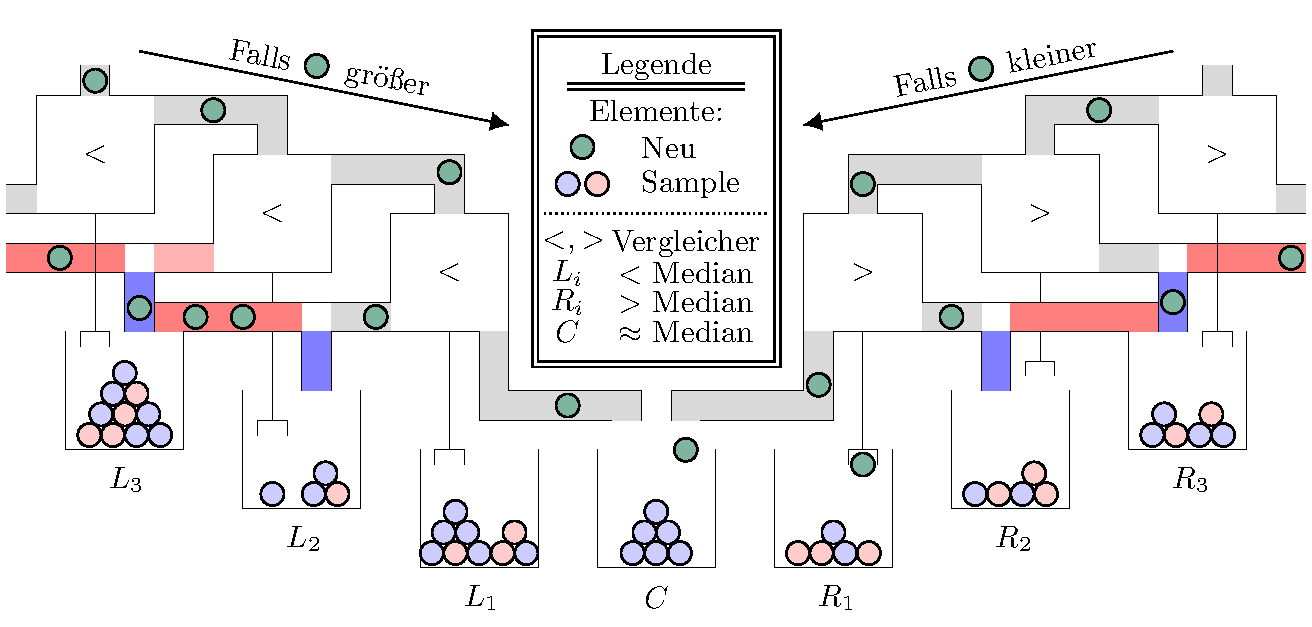
\includegraphics[scale=2]{pics/rmedian}
    \vspace*{-0.5cm}
    \captionof{figure}{\textit{RMedian}, Schritt 2: Einteilung neuer 
    Elemente durch Vergleiche mit Elementen aus den Buckets $L_i, C, R_i$}
    \vspace*{.4cm}
\end{center}

\noindent
\textcolor{black}{
Zunächst wird ein randomisiertes Sample gewählt und sortiert. 
Hieraus werden nun repräsentative Mengen für Elemente kleiner, größer 
oder in der Nähe des Medians erwartet. 
Wie in Abbildung 1 zu sehen, werden nun alle weiteren Elemente nacheinander 
mit Elementen der einzelnen Buckets verglichen und entsprechend einsortiert.\\
Die Mengen $L_i$ beinhalten hierbei jene Elemente, die kleiner als der Median vermutet 
werden und die Mengen $R_i$ analog Elemente größer als der Median. 
In der Menge $C$ befinden sich abschließend alle Mediankandidaten.
}\\
\color{goetheblau}{\rule{\textwidth}{0.1cm}}
% ================================================================
% COL 2
% ================================================================
% Column Left
\begin{multicols}{2}
\section{RMinimum \& RMedian}
\vspace*{-0.05cm}
\noindent
\textcolor{black}{
Beide Algorithmen erhalten als Eingabe eine total geordnete Menge $X$ 
mit Mächtigkeit $n$ sowie einen sogenannten \textit{Tuningparameter} $k(n)$, 
mit dessen Hilfe sich ein \textit{Trade-off} zwischen der erwarteten 
\fg $f_{min}(n)$ des Minimums beziehungsweise $f_{med}$ des Medians sowie der 
erwarteten \fg $f_{rem}(n)$ aller übrigen Elemente regulieren lässt. 
Eine elementare Idee beider Algorithmen ist es hierbei eine randomisierte Teilmenge 
der Eingabemenge zu wählen und diese als Sample für weitere Vergleiche zu nutzen.
Durch ihren Aufbau nehmen Elemente bei zunehmender Distanz zum 
Minimum bzw. Median häufiger an Vergleichen teil. Die Analyse der Arbeit beschränkt sich im wesentlichen auf gegebene 
Abschätzungen der Paare $<\mathbb{E}[f_{min/med}],\mathbb{E}[f_{rem}]>$.}
% --------------------------------
% Theorem 5
\begin{manualtheorem}{1}
    \textcolor{black}{
    Sei $k(n)=\log(n)/\log\log(n)$. Dann benötigt \Rm $\mathbb{E}[f_{min}]=\mathcal{O}(\log(n)/\log\log(n))$ Vergleiche für das Minimum Element und $\mathbb{E}[f_{rem}]=\mathcal{O}(\log(n)/\log\log(n))$ für alle übrigen Elemente.}
\end{manualtheorem}

% --------------------------------
\noindent
\textcolor{black}{
Wie in Abbildung 2 zu sehen konnte für alle nicht-median Elemente ein passender \textit{Fit} der Form $F(n) = a \cdot \log(n)/ \log\log(n) + b$ gefunden werden.}

% --------------------------------
% Figure 2 - RMin Analyse
\begin{center}
    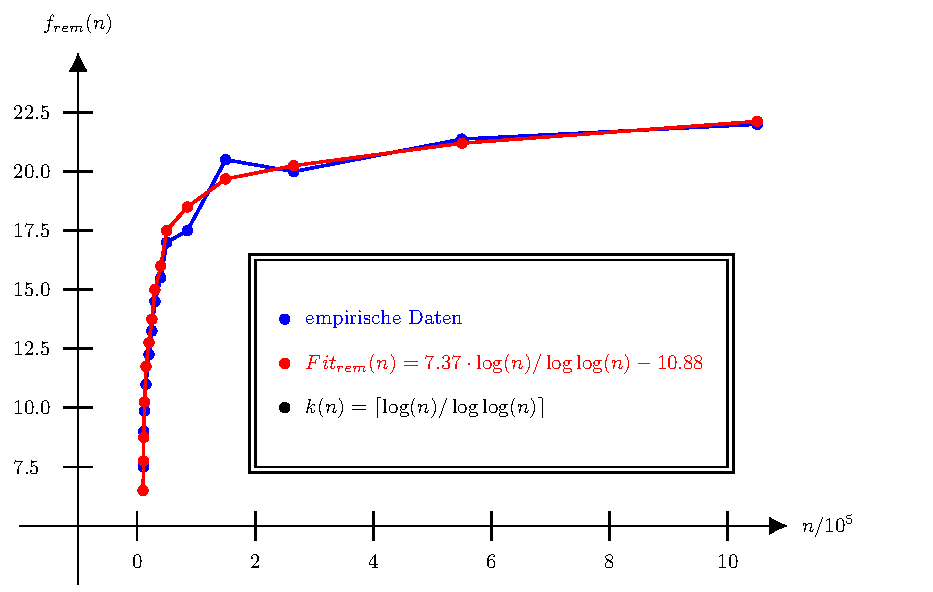
\includegraphics[scale=1.5]{pics/theo5_rem}
    \vspace*{-2cm}
    \captionof{figure}{Fit für $f_{min}$ für \Rm}
\end{center}
% --------------------------------
\noindent
\textcolor{black}{
Für beide Algorithmen konnte zudem bestätigt werden, dass die Anzahl 
der insgesamt benötigten Vergleiche linear in der Eingabegröße ist.}

% --------------------------------
% Section


\end{multicols}
\end{document}
% ================================================================
